% -*- coding: utf-8 -*-
% 自然语言处理作业一实验报告（南开大学计算机学院 LaTeX 模板）
\documentclass[UTF8,a4paper,10pt]{ctexart}
\usepackage[left=3.17cm, right=3.17cm, top=2.74cm, bottom=2.74cm]{geometry}
\usepackage{amsmath}
\usepackage{graphicx,subfig}
\usepackage{float}
\usepackage{cite}
\usepackage{caption}
\usepackage{enumerate}
\usepackage{booktabs} %表格
\usepackage{multirow}
\newcommand{\tabincell}[2]{\begin{tabular}{@{}#1@{}}#2\end{tabular}}  %表格强制换行
%-------------------------字体设置--------------
\usepackage{ctex}
\setCJKmainfont[Path=/root/fonts/, BoldFont=NotoSerifCJKSCBold.otf]{NotoSerifCJKSC.otf}
\newcommand{\yihao}{\fontsize{26pt}{36pt}\selectfont}           % 一号, 1.4 倍行距
\newcommand{\erhao}{\fontsize{22pt}{28pt}\selectfont}          % 二号, 1.25倍行距
\newcommand{\xiaoer}{\fontsize{18pt}{18pt}\selectfont}          % 小二, 单倍行距
\newcommand{\sanhao}{\fontsize{16pt}{24pt}\selectfont}  %三号字
\newcommand{\xiaosan}{\fontsize{15pt}{22pt}\selectfont}        % 小三, 1.5倍行距
\newcommand{\sihao}{\fontsize{14pt}{21pt}\selectfont}            % 四号, 1.5 倍行距
\newcommand{\banxiaosi}{\fontsize{13pt}{19.5pt}\selectfont}    % 半小四, 1.5倍行距
\newcommand{\xiaosi}{\fontsize{12pt}{18pt}\selectfont}            % 小四, 1.5倍行距
\newcommand{\dawuhao}{\fontsize{11pt}{11pt}\selectfont}       % 大五号, 单倍行距
\newcommand{\wuhao}{\fontsize{10.5pt}{15.75pt}\selectfont}    % 五号, 单倍行距
%-------------------------章节名----------------
\usepackage{ctexcap}
\CTEXsetup[name={,、},number={ \chinese{section}}]{section}
\CTEXsetup[name={（,）},number={\chinese{subsection}}]{subsection}
\CTEXsetup[name={,.},number={\arabic{subsubsection}}]{subsubsection}
%-------------------------页眉页脚--------------
\usepackage{fancyhdr}
\pagestyle{fancy}
\lhead{\kaishu \leftmark}
\rhead{\kaishu 自然语言处理实验报告}
\lfoot{}
\cfoot{\thepage}
\rfoot{}
\renewcommand{\headrulewidth}{0.1pt}
\renewcommand{\footrulewidth}{0pt}
\newcommand{\HRule}{\rule{\linewidth}{0.5mm}}
%------------------------代码-------------------
\usepackage{xcolor}
\usepackage{listings}
\lstset{
breaklines,
basicstyle=\small\ttfamily,
escapeinside=``,
keywordstyle=\color{blue!70}\bfseries,
commentstyle=\color{red!50!green!50!blue!50},
stringstyle=\ttfamily,
extendedchars=false,
linewidth=\textwidth,
numbers=left,
numberstyle=\tiny\color{blue!50},
frame=trbl
}
%------------超链接----------
\usepackage[colorlinks,linkcolor=black,anchorcolor=blue]{hyperref}
\hypersetup{pdftitle={自然语言处理作业一实验报告：文本分类实现},pdfauthor={吴嘉豪}}
%------------------------枚举符号-------------------
\usepackage{enumitem,amssymb}
\usepackage{needspace}
\usepackage{pifont}
\newcommand{\cmark}{\ding{51}}%
\newcommand{\xmark}{\ding{55}}%
%------------------------水印-------------------
\usepackage{tikz}
\usepackage{xcolor}
\usepackage{eso-pic}
\newcommand{\watermark}[3]{\AddToShipoutPictureBG{
\parbox[b][\paperheight]{\paperwidth}{
\vfill%
\centering%
\tikz[remember picture, overlay]%
  \node [rotate = #1, scale = #2] at (current page.center)%
    {\textcolor{gray!80!cyan!30!magenta!30}{#3}};
\vfill}}}

%———————————————————————————————————————————正文———
\begin{document}
\begin{titlepage}
    \begin{center}
    
\includegraphics[width=0.8\textwidth]{NKU.png}\\[1cm]
    \textsc{\Huge \kaishu{\textbf{南\ \ \ \ \ \ 开\ \ \ \ \ \ 大\ \ \ \ \ \ 学}} }\\[0.9cm]
    \textsc{\huge \kaishu{\textbf{计\ \ 算\ \ 机\ \ 学\ \ 院}}}\\[0.5cm]
    \textsc{\Large \textbf{自然语言处理课程作业一}}\\[0.8cm]
    \HRule \\[0.9cm]
    { \LARGE \bfseries 文本分类实现：词袋、词向量与 BERT 的对比实验}\\[0.4cm]
    \HRule \\[2.0cm]
    \centering
    \textsc{\LARGE \kaishu{姓名\ :\ 吴嘉豪}}\\[0.5cm]
    \textsc{\LARGE \kaishu{学号\ :\ 2113454}}\\[0.5cm]
    \textsc{\LARGE \kaishu{年级\ :\ 2021级}}\\[0.5cm]
    \textsc{\LARGE \kaishu{专业\ :\ 计算机科学与技术}}\\[0.5cm]
    \vfill
    {\Large \today}
    \end{center}
\end{titlepage}
%-------------摘------要--------------
\newpage
\thispagestyle{empty}
\renewcommand{\abstractname}{\kaishu \sihao \textbf{摘要}}
    \begin{abstract}

        \noindent
        本报告在 New York Times（NYT）新闻数据集的 business、politics、sports 三个类别上完成文本分类任务。
        我们对比了三类文本表示方法：Binary Bag-of-Words 与 Word Frequency 两种稀疏表示、三组 100 维词向量的
        平均池化表示（预训练 GloVe、以 AG News 语料训练的 Word2Vec、以 NYT 训练集训练的 Word2Vec），以及微调的
        bert-base-uncased 预训练语言模型。所有实验使用同一份 80\%/10\%/10\% 数据划分，统一以 Accuracy 与
        Macro-F1 在相同测试集上评价。结果表明：Word Frequency 加 Logistic Regression 取得最好效果
        （Accuracy 0.9913 / Macro-F1 0.9817）；平均池化的词向量表示整体低约 1 个百分点，其中语料与任务匹配度
        比语料规模的影响更大；BERT 微调是最好的神经方法（Accuracy 0.9844 / Macro-F1 0.9676），但在该数据
        规模上未超过线性词袋基线。类别不均衡使得 Accuracy 与 Macro-F1 之间始终存在 1--3 个百分点的差距，
        两项指标需要同时报告。

        \vspace{0.5em}
        \noindent
        \textbf{关键词：}文本分类；词袋模型；Word2Vec；GloVe；BERT；Logistic Regression
    \end{abstract}
%----------------------------------------------------------------
\tableofcontents
%----------------------------------------------------------------
\newpage
\watermark{60}{10}{NKU}
\setcounter{page}{1}

\section{实验概述}
本实验在 New York Times（NYT）新闻数据集上完成文本分类任务。数据集包含 business、politics、sports 三个类别，类别分布不均衡（sports 约占 75\%）。实验分别使用三类文本表示方法训练分类器，并在完全相同的数据划分上比较性能：

\begin{enumerate}
  \item \textbf{词袋模型（Task 1，30 分）}：Binary Bag-of-Words 与 Word Frequency 两种稀疏表示 + Logistic Regression；
  \item \textbf{词向量（Task 2，50 分）}：预训练 GloVe\cite{pennington2014glove}、AG News 自训练 Word2Vec\cite{mikolov2013word2vec} 与 NYT 自训练 Word2Vec，文档向量取词向量平均 + Logistic Regression；
  \item \textbf{预训练语言模型（Task 3，20 分）}：微调 bert-base-uncased\cite{devlin2019bert}，max\_length=64，3 epochs。
\end{enumerate}

评价指标为 Accuracy 与 Macro-F1。由于类别不均衡，少数类（business / politics）的识别能力在 Accuracy 中容易被掩盖，Macro-F1 通过对各类别 F1 取平均提供更公平的度量。

实验环境为 Windows 10，NVIDIA RTX 3050 Laptop 4GB，Python 3.12，scikit-learn 1.9、gensim 4.4、nltk 3.10、PyTorch 2.14（CUDA 12.6）、transformers 5.17；BERT 微调使用 fp16 混合精度，batch size 16。

\section{数据集与预处理}

\subsection{数据划分}
NYT 数据集共 11,519 篇新闻（text + label 两列），作为分类主数据集；AG News 数据集共 90,000 篇文本（仅 text 一列，无标签），仅用于 Task 2 中训练 Word2Vec 词向量。

对 NYT 全量数据以固定随机种子（random\_state=42）随机打乱后，按 80\% / 10\% / 10\% 划分训练集、验证集与测试集。划分采用分层抽样，保持各类别比例一致；划分结果落盘保存，所有实验加载同一份数据，保证方法间的可比性。验证集仅用于超参数选择（如 BERT 学习率），测试集仅用于最终性能报告，各类别分布见表~\ref{tab:split}。

\begin{table}[!htbp]
  \centering
  \begin{tabular}{lccccc}
  \toprule
  划分 & 样本数 & business & politics & sports \\
  \midrule
  Training   & 9,215 & 1,143 & 1,161 & 6,911 \\
  Validation & 1,152 &   143 &   145 &   864 \\
  Test       & 1,152 &   143 &   145 &   864 \\
  \bottomrule
  \end{tabular}
  \caption{NYT 数据集 80/10/10 划分及类别分布（分层，随机种子 42）}
  \label{tab:split}
\end{table}

\subsection{分词}
全流程统一使用 nltk.word\_tokenize 分词：先小写化，再仅保留纯字母 token（去除数字与标点，这类 token 无对应词向量且对分类贡献很小）。同一分词方案用于 BoW 词表构建、Word2Vec 训练语料与文档向量计算，保证各方法输入一致。

\section{Task 1：Bag of Words + Logistic Regression}

从训练集构建词表，$|V| = 57{,}275$。每篇文档表示为 $|V|$ 维向量，两种表示的区别仅在于分量取值：Binary BoW 记录词是否出现（取 0/1），Word Frequency 记录词出现次数。两种表示均以 scikit-learn 的 CountVectorizer 实现（binary=True/False），分类器统一为 LogisticRegression（max\_iter=1000）。结果见表~\ref{tab:task1}。

\begin{table}[!htbp]
  \centering
  \begin{tabular}{lcc}
  \toprule
  表示方法 & Accuracy & Macro-F1 \\
  \midrule
  Binary BoW     & 0.9905 & 0.9775 \\
  Word Frequency & \textbf{0.9913} & \textbf{0.9817} \\
  \bottomrule
  \end{tabular}
  \caption{两种词袋表示的分类性能（NYT Test Set）}
  \label{tab:task1}
\end{table}

两种 BoW 表示均达到约 99\% 的准确率，说明该任务中“哪些词出现”本身就是很强的分类信号（比如 sports 类的 team、game、season 这类词）。词频版略优于二值版，说明出现次数提供了额外的强度信息。但新闻文本中多数词仅出现一次，因此两者差距很小（Accuracy 相差 0.0008）。

\section{Task 2：词向量 + Logistic Regression}

统一使用 100 维词向量；文档向量 = 文档内所有有效单词词向量的平均（测试集中不存在完全无词表命中的退化样本）。三组实验的区别仅在词向量来源：

\begin{enumerate}
  \item \textbf{预训练 GloVe}：官方 glove.6B.100d.txt（400,000 词，60 亿词符语料训练）；
  \item \textbf{Word2Vec（AG News）}：gensim Word2Vec，vector\_size=100、window=5、min\_count=5、CBOW、5 epochs，在 AG News 全量 90,000 篇上训练；
  \item \textbf{Word2Vec（NYT）}：同超参数，仅在 NYT 训练集（9,215 篇）上训练，严格将验证与测试数据排除在一切训练过程之外。
\end{enumerate}

\begin{table}[!htbp]
  \centering
  \begin{tabular}{lcc}
  \toprule
  文档表示 & Accuracy & Macro-F1 \\
  \midrule
  GloVe 6B 100d（预训练）     & 0.9800 & 0.9526 \\
  Word2Vec 训练于 AG News     & 0.9792 & 0.9500 \\
  Word2Vec 训练于 NYT         & \textbf{0.9809} & \textbf{0.9540} \\
  \bottomrule
  \end{tabular}
  \caption{三种词向量文档表示的分类性能（NYT Test Set）}
  \label{tab:task2}
\end{table}

\subsection{定性检查：最近邻词}

对两个自训练 Word2Vec 模型查询典型词的最近邻（表~\ref{tab:nn}），可以直观看出训练语料领域的影响。

\begin{table}[!htbp]
  \centering
  \small
  \begin{tabular}{lll}
  \toprule
  查询词 & W2V-AG News 最近邻 & W2V-NYT 最近邻 \\
  \midrule
  president & administration, leader, dushanbe, voltchkov & chairman, secretary, chairwoman, adviser, barack \\
  baseball  & franchise, owners, nfl, selig              & mlb, rivera, rodriguez, yankees \\
  economy   & economic, recovery, inflation, growth, currency & growth, inflation, economic, market, crisis \\
  \bottomrule
  \end{tabular}
  \caption{两个自训练 Word2Vec 模型的最近邻词（余弦相似度）}
  \label{tab:nn}
\end{table}

\subsection{分析}

平均词向量方法整体比 BoW 低约 1 个百分点。平均操作把整篇文档压缩成 100 维，抹平了词序与关键词的尖峰信号；BoW 的 57,275 维稀疏向量则保留了每个判别性词汇的独立权重，而 Logistic Regression 恰好擅长利用这种稀疏线性结构。

W2V-NYT 的训练语料只有 AG News 的约 1/10，分类性能却略高一些。从表~\ref{tab:nn} 的最近邻看，NYT 训练出的向量更贴近该数据集自身的时政与体育词汇，barack、yankees 等正是本任务的强判别词；AG 语料以短财经、体育快讯为主，向量里混进了网球选手这类与 NYT 无关的实体。对平均池化来说，语料的词分布与下游任务是否接近，比语料规模的影响更大。

预训练 GloVe 的表现与 NYT 自训练的 Word2Vec 基本持平（Macro-F1 相差 0.0014）。GloVe 的训练语料大了两个数量级，但并不偏向 NYT 的词汇分布，规模优势没有体现出来，与上面的观察一致。

\section{Task 3：BERT 微调}

以 AutoModelForSequenceClassification 加载 google-bert/bert-base-uncased（12 层、768 维、约 1.1 亿参数）并接三分类头。Tokenization 设 max\_length=64 并截断，训练时以 DataCollatorWithPadding 按 batch 动态补齐。训练共 3 个 epoch，batch size 16，采用 AdamW 优化器与线性 warmup 调度，并以 fp16 混合精度训练。学习率按 BERT 论文\cite{devlin2019bert}推荐值在验证集上从 \{2e-5, 3e-5\} 中选择，结果见表~\ref{tab:bert}。

\begin{table}[!htbp]
  \centering
  \begin{tabular}{lcccc}
  \toprule
  学习率 & Val Accuracy & Val Macro-F1 & Test Accuracy & Test Macro-F1 \\
  \midrule
  2e-5 & 0.9792 & 0.9530 & 0.9844 & 0.9657 \\
  \textbf{3e-5（选用）} & \textbf{0.9800} & \textbf{0.9553} & \textbf{0.9844} & \textbf{0.9676} \\
  \bottomrule
  \end{tabular}
  \caption{BERT 微调学习率对比（最终模型按验证集 Macro-F1 选出）}
  \label{tab:bert}
\end{table}

\subsection{分析}

训练损失在 3 个 epoch 内降到 0.01 左右，基本记住了训练集。微调后 BERT 的 98.44\% 准确率高于三种平均词向量方法（97.9\%--98.1\%），说明上下文相关的表示和端到端微调确实带来了提升：注意力可以聚焦关键短语，而不是被大量次要词的平均稀释。

测试集错误集中在 politics 类（recall 约 0.92--0.96），该类与 business 共享大量经济政策词汇，是三个类别中最难区分的一对。在 9,215 篇的小训练集上，BERT 未超过 BoW + LR 基线（99.13\%）；学习率从 2e-5 提高到 3e-5 仅带来 0.002 的 Macro-F1 提升，说明模型已接近数据量约束下的上限。此外，作业固定要求 max\_length=64，对 NYT 长文本存在信息截断，也是其相对 BoW 的一个不利因素。

\section{总体比较与讨论}

全部 7 组实验在相同数据划分上的测试集性能汇总见图~\ref{fig:methods} 与表~\ref{tab:all}。

\begin{figure}[H]
    \centering
    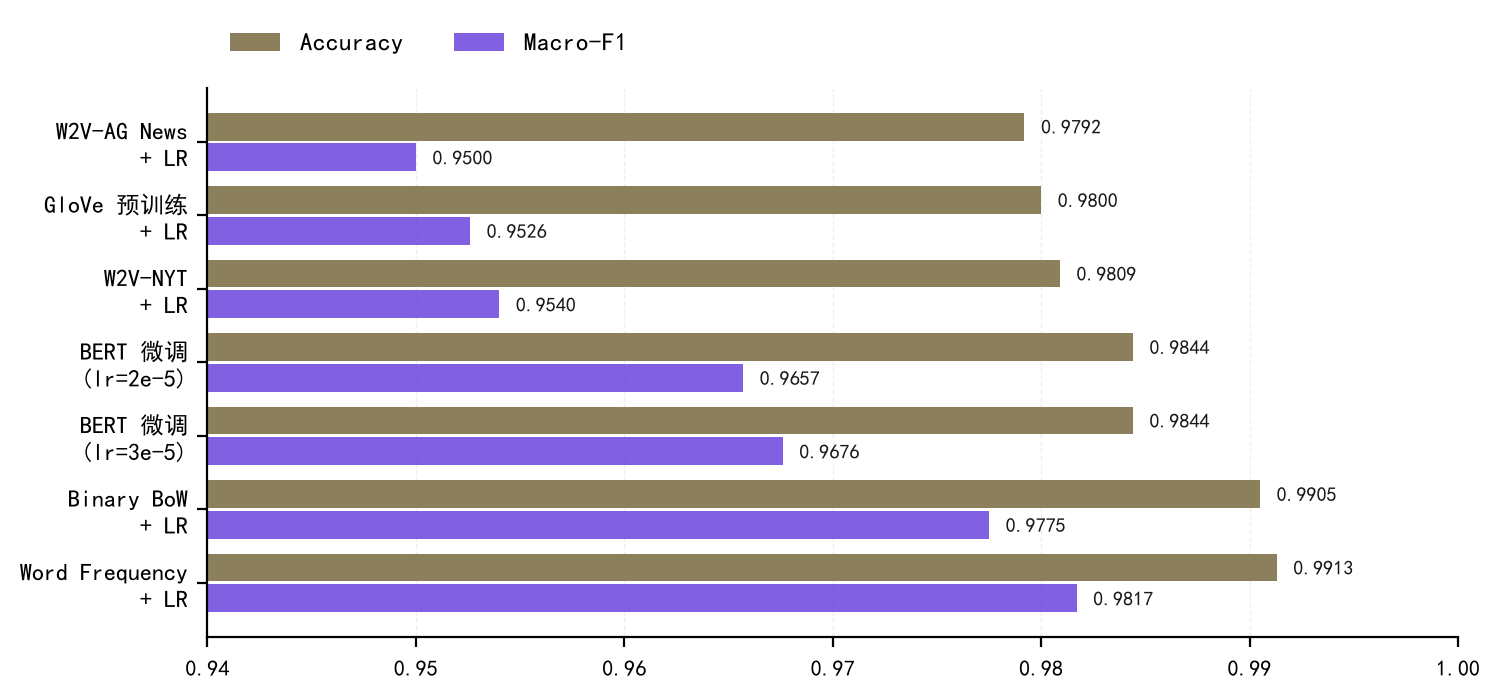
\includegraphics[width=0.98\textwidth]{chart_methods.png}
    \caption{七组实验的 Test Accuracy 与 Macro-F1 对比}
    \label{fig:methods}
\end{figure}

\begin{table}[!htbp]
  \centering
  \small
  \begin{tabular}{lcc}
  \toprule
  实验设置 & Accuracy & Macro-F1 \\
  \midrule
  Task1: Binary BoW + LR                    & 0.9905 & 0.9775 \\
  Task1: Word Frequency + LR                & \textbf{0.9913} & \textbf{0.9817} \\
  Task2a: GloVe 6B 100d（平均）+ LR         & 0.9800 & 0.9526 \\
  Task2b: Word2Vec（AG News 训练，平均）+ LR & 0.9792 & 0.9500 \\
  Task2c: Word2Vec（NYT 训练，平均）+ LR     & 0.9809 & 0.9540 \\
  Task3: BERT 微调（lr=2e-5）               & 0.9844 & 0.9657 \\
  Task3: BERT 微调（lr=3e-5，最终）         & 0.9844 & 0.9676 \\
  \bottomrule
  \end{tabular}
  \caption{全部实验的性能汇总（NYT Test Set，相同 80/10/10 划分，最优值加粗）}
  \label{tab:all}
\end{table}

效果最好的仍然是最简单的词袋表示。这个任务里每类都有大量强特征词，类别间接近线性可分，BoW 加 Logistic Regression 因此很难被超越。深度模型的优势需要足够多的训练数据才能发挥，本任务的训练集只有 9,215 篇。

三组词向量实验的结果非常接近，瓶颈应该在平均池化这种表示方式本身：求平均时会丢失词序和关键句的信息，静态向量也处理不了多义词，换不同的训练语料带来的改善有限。

BERT 微调超过了全部三组平均词向量方法，是表现最好的神经方法，但仍没有超过线性基线，这与文献中“强线性基线难以击败”的观察相符。

所有方法的 Accuracy 都比 Macro-F1 高 1 到 3 个百分点，差距来自 sports 占约 75\% 的类别不均衡：多数类的正确预测抬高了 Accuracy，而少数类的少量错误在 Macro-F1 中被明显放大，所以评价这类数据时两项指标都要看。

\needspace{14\baselineskip}
\section{总结}

\begin{enumerate}
  \item Word Frequency + Logistic Regression 取得了最好的结果（Accuracy 0.9913 / Macro-F1 0.9817），Binary BoW 紧随其后。对这个线性可分性较好的新闻分类任务，稀疏词袋特征已经足够有效。
  \item 三种词向量文档表示性能相近，整体比 BoW 低约 1 个百分点；其中在规模小得多的 NYT 语料上训练的 Word2Vec 反而优于 AG News 语料训练的版本，说明语料与任务的匹配程度比规模更重要。
  \item BERT 微调（Accuracy 0.9844 / Macro-F1 0.9676）是最好的神经方法，说明预训练模型对上下文语义的建模有价值，但在本数据规模上没有超过线性基线。
  \item Accuracy 与 Macro-F1 的差距来自类别不均衡，少数类的错误对 Macro-F1 影响更大，评价不均衡数据时两项指标都应报告。
\end{enumerate}

\newpage
\section{附录：复现说明}

完整代码与依赖清单见 hw1/ 目录与仓库根目录 requirements.txt，运行说明见 hw1/README.md。以下命令均在 hw1/ 目录下执行：

\begin{lstlisting}[title=运行顺序,frame=trbl,language={bash}]
python src/data_prep.py          # 生成固定数据划分
python src/task1_bow.py          # Task 1: Binary BoW / Word Frequency + LR
python src/task2_word2vec.py     # Task 2b/2c: Word2Vec(AG / NYT) + LR
python src/task2_glove.py        # Task 2a: GloVe 6B 100d + LR
python src/task3_bert.py --lr 3e-5   # Task 3: BERT 微调（学习率可选）
python src/aggregate_results.py  # 汇总 results/results.csv
\end{lstlisting}

GloVe 下载自 \href{http://nlp.stanford.edu/data/glove.6B.zip}{nlp.stanford.edu/data/glove.6B.zip}（解压出 glove.6B.100d.txt 放入 data/ 目录）；BERT 权重本地缓存于 models/bert-base-uncased/（SHA256 已与官方发布核对一致）；NLTK 分词数据需一次性 nltk.download("punkt") 与 nltk.download("punkt\_tab")。

代码结构：本仓库按作业组织，每次作业独立放在 hw1/、hw2/ 等文件夹中。hw1/src/common.py 提供共享工具（数据加载、分词、平均池化、评估与结果落盘），保证各任务使用完全相同的数据划分与评价流程；data\_prep.py 生成并落盘 80/10/10 划分；各 task 脚本分别实现对应任务；aggregate\_results.py 汇总所有实验指标（hw1/results/results.csv）。hw1/data/raw/ 存放原始数据，hw1/report/ 存放本报告。

%----------------------------------------------------------------
\newpage
\bibliographystyle{plain}
\bibliography{references}
\end{document}
